\documentclass[
  % all of the below options are optional and can be left out
  % course name (default: 2IL50 Data Structures)
  course = {{Electricity and Magnetism 3}},
  % quartile (default: 3)
  term = {{4a Fall 2020}},
  % assignment number/name (default: 1)
  assignment = 1,
  % student name (default: Some One)
  name = {{Andrew Kovachik}},
  % student number, NOT S-number (default: 0123456)
  studentnumber = {{20673849}},
  % student email (default: s.one@student.tue.nl)
  email = {{kovachik.andrew@gmail.com ; ajkovach@uwaterloo.ca}},
  % first exercise number (default: 1)
  firstexercise = 1
]{aga-homework}

\usepackage{physics}
\usepackage{graphicx}
\graphicspath{{./figures/}}

\begin{document}


\exercise

\subexercise

A parallel plate capacitor is formed of two flat rectangular perfectly conducting sheets of
dimensions $a$ and $b$ separated by a distance $d$, which is small compared to $a$ or $b$. Current
is fed in and taken out uniformly along adjacent edges of length $b$. With time-harmonic input
current and voltage defined at this end of the capacitor:

\ssubexercise

Calculate the input impedance or admittance.


\ssubexercise

Calculate the electric and magnetic fields in the capacitor correct to second order in powers of the
frequency $\omega$, but neglecting fringing fields.

Hint:

$$
E = E_0 + \omega E_1+ \omega^2 E_2 + \dots
$$
$$
B = B_0 + \omega B_1+ \omega^2 B_2 + \dots
$$
$$
\vb{E}(y) = E(y)e^{-iwt}\vu{k}
$$
$$
\vb{B}(y) = B(y)e^{-iwt}\vu{y}
$$

\newpage
\subexercise

\begin{figure}[h]
    \centering
    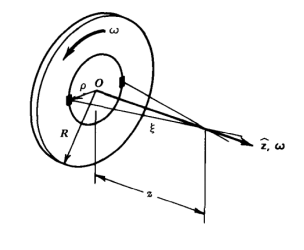
\includegraphics[width=0.5\textwidth]{disk}
    \caption{Diagram for question 1b}
    \label{disk}
\end{figure}

A uniformly charged thin disk of charge density $\sigma$, radius $R$, and thickness $t<R$ rotates
with an angular velocity $w$ about the $z$ axis of symmetry, as shown in figure \ref{disk}. 

\ssubexercise

Find the magnetic field at the point located on the $z$ axis of symmetry.

\ssubexercise

Obtain the solution for a sphere of volume charge density $\rho_0$ and the same radius.


\newpage
\subexercise

\begin{figure}[h]
    \centering
    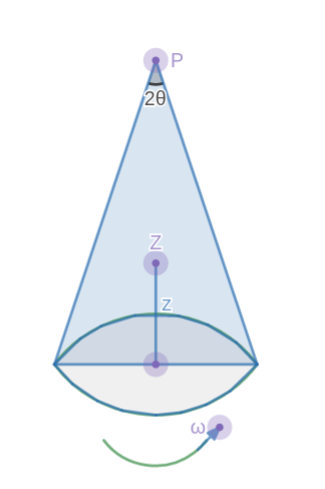
\includegraphics[width=0.3\textwidth]{cone}
    \caption{Diagram for question 1c}
    \label{cone}
\end{figure}

A hollow cone (like a party hat!) has a vertex angle, $2\theta_0$. The radius on the base is $R$ and
the height is $H$. It has a surface charge density, $\rho$. It spins around its symmetric axis with
angular frequency $\omega$. What is the magnetic field at the top vertex (point P) and the point $Z$
at the distance $z$ from the bottom?


\newpage
\exercise

\subexercise

\begin{figure}[h]
    \centering
    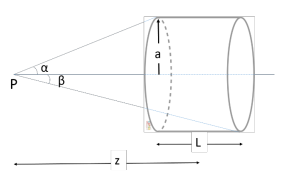
\includegraphics[width=0.5\textwidth]{solenoid}
    \caption{Diagram for question 2a}
    \label{solenoid}
\end{figure}
The magnetic field due to a ring of current of radius $a$, distance $z$ away on the axis of the ring
is given by $\frac{\mu_0I}{2a} sin^3(\theta)$, $tan\theta = a/z$.  You may use this result in your
calculations. Consider a short, (not ideal) solenoid as shown in the figure \ref{solenoid}, of length $L$, numbmer
of turns per unit length $n$, radius $a$, and current $I$ flowing through its turns.

\ssubexercise

Find the magnetic field due to the short solenoid, on the axis of the solenoid, on the axis of the
solenoid at the point $P$ at a distance $z$ away from the center of the solenoid. $P$ is outside the
solenoid. Give the answer in terms of the angles $\alpha$ and $\beta$, where $\alpha$ and $\beta$
are defined in the figure.

\ssubexercise

Find the magnetic field at the center of the short solenoid when the diameter of the solenoid is
equal to its length.

\ssubexercise

Find the limit of the field at the center of the solenoid when the length of the solenoid is much
larger than the diameter. Is this what you expect? Explain.

\ssubexercise

Does Ampere's law hold for the case of the short solenoid? Explain and elaborate.

\newpage
\subexercise


\ssubexercise

Show that the energy of the magnetic field of a stationary current distribution $\vec{j}(\vec{x})$
in vaccum is determined by:

$$
W = \frac{1}{2c^2} \int d^3\vec{x} \int d^3\vec{x}' \frac{\vec{j}(\vec{x})\dot
\vec{j}(\vec{x}')}{\abs{\vec{x}-\vec{x}'}}
$$


\ssubexercise

The energy of a system of $n$ current carrying conductors (current $I_i$) can be described by the
quadratic form 

$$
W = \frac{1}{2} \sum\limits_{i=1}^n L_i I_i^2 + \sum\limits_{i=1}^n\sum\limits_{j>i}^n L_{ij} I_i
I_j
$$


Find the expression for the self-induction coefficients $L_i$ and the mutual induction coefficients,
$L_{ij}$.

\ssubexercise

\begin{figure}[h]
    \centering
    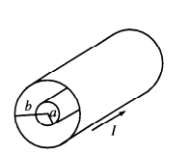
\includegraphics[width=0.25\textwidth]{cyl}
    \caption{Diamgram for 2b}
    \label{cyl}
\end{figure}

Calculate the self-induction coefficient in (b) for a long current-carrying coaxial line (as in
figure \ref{cyl}). Let the inner conductor (radius $a$) have the permeability, $\mu_0$. The space
between the conductors should be filled with a material of permeability, $\mu$.

\newpage
\subexercise

A solenoid of radius $R$ with $n$ turns per unit length, carries a stationary current, $I$. Two
hollow cylinders of length $l$ are fixed coaxially and freely rotation. One cylinder of radius, $a$,
is insider the coil ($a<R$) and carries the uniformly distributed charge, $Q$. The other cylinder of
radius, $b$ ($b>R$) carries the carge, $-Q$. If the current is switched off the cylinders start to
rotate. What is the value of the angular momentum? Where does the angular momentum come from?
\end{document}

